\documentclass{beamer}
 
\usepackage[utf8]{inputenc}
\usepackage{lmodern}% http://ctan.org/pkg/lm

% for table formatting
\usepackage{multirow}
\usepackage{color,soul}
\usepackage{array}
\newcolumntype{L}[1]{>{\raggedright\let\newline\\\arraybackslash\hspace{0pt}}m{#1}}
 
% TITLE PAGE -------------------------------------------------------

\title{Predicting Airbnb User Booking Destinations}
\author{Lisa Oshita\\Dr. Glanz}

\begin{document}
 
\frame{\titlepage}

% BACKGROUND INFO -------------------------------------------------

\begin{frame}
\frametitle{About the Competition}
  \begin{itemize}
    \item Recruiting competition hosted on Kaggle from November 2015 to February 2016 \vspace{1ex}
    \item \textbf{Task:} build a model to predict where new Airbnb users will book their first destinations \vspace{1ex}
    \item \textbf{12 possible destinations to predict:} Australia, Canada, France, Germany, Italy, Netherlands, Portugal, Spain, United Kingdom, US, other and no destination found (NDF)
  \end{itemize}
\end{frame}

% ABOUT THE DATA --------------------------------------------------

\begin{frame}
\frametitle{About the Data}
\begin{itemize}
  \item \textbf{train\_users} 
  \begin{itemize}
    \item 213,415 observations and 16 variables
    \item Contains information about users from 2010 to 2014 \vspace{2ex}
  \end{itemize}
  \item \textbf{sessions}
  \begin{itemize}
    \item 1,048,575 rows and 12,994 unique users
    \item contains information about web session activity for each user
    \item 10\% of rows from each unique user were randomly sampled
    \item New sampled data contained 104,424 rows  
  \end{itemize}
\end{itemize}
\end{frame}

% MODELS EXPLORED -------------------------------------------------

\begin{frame}
\frametitle{Models}
  \begin{itemize}
    \item Extreme Gradient Boosting (XGBoost)
    \item Random forest
    \item Stacked model
  \end{itemize}
\end{frame}

% FEATURE ENGINEERING ---------------------------------------------

\begin{frame}
\frametitle{Feature Engineering}
\begin{itemize}
  \item Date features
  \item Age and gender
  \item Count features created from the sessions data (e.g. number of times a user viewed recent reservations, number of times a user viewed similar listings...)
  \item Summary statistics of seconds elapsed for each user’s web session
\end{itemize}
\end{frame}

% IMBALANCED CLASSES ----------------------------------------------

\begin{frame}
\frametitle{Booking Destinations: Extremely Imbalanced Classes}
\begin{columns}
  \begin{column}{0.45\textwidth}
      \begin{figure}
        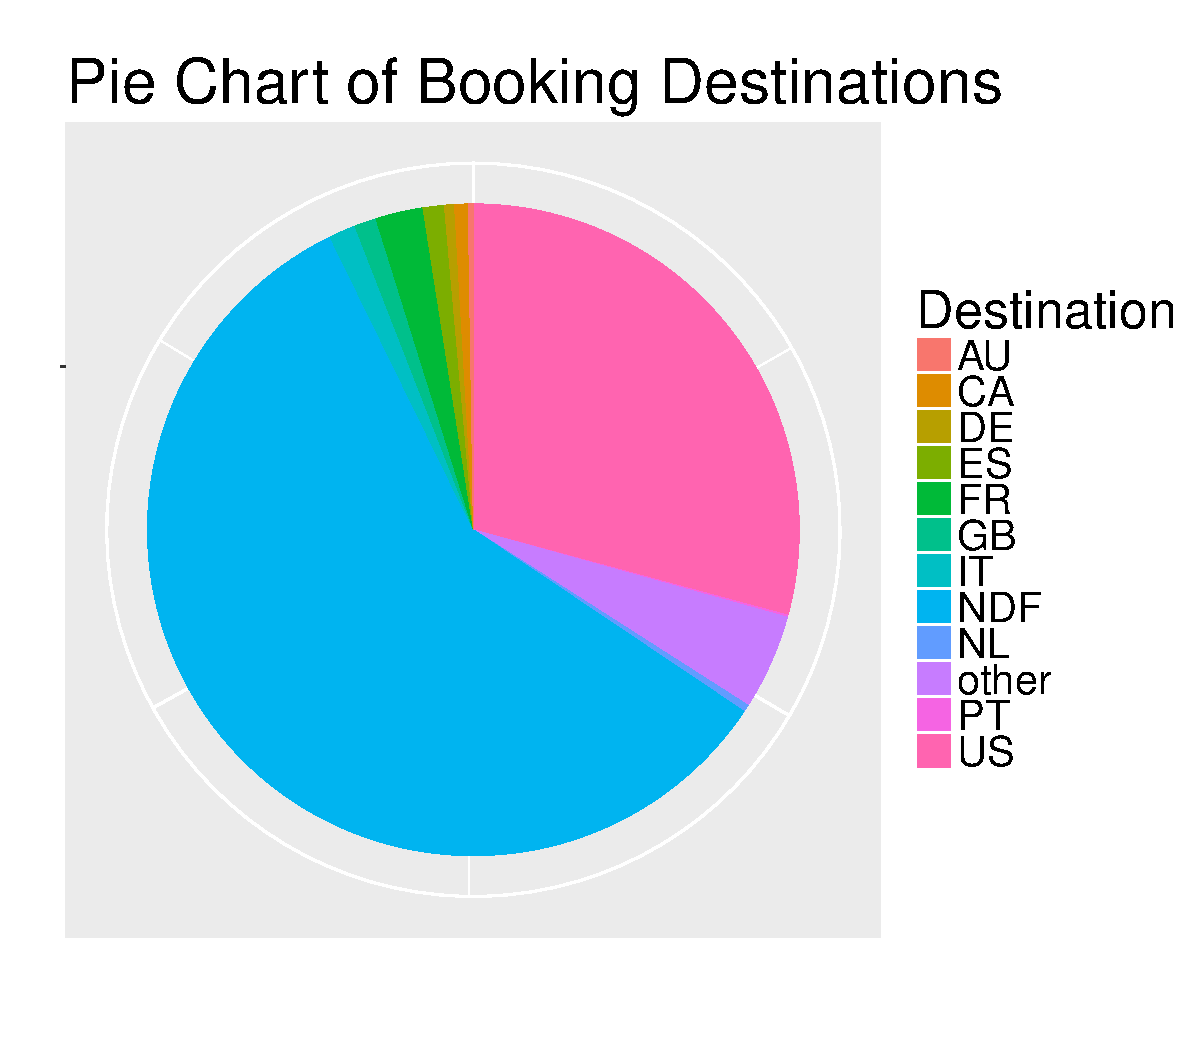
\includegraphics[width = 1.0\textwidth]{pie_chart_dest.pdf} 
      \end{figure}
  \end{column}
  \begin{column}{0.55\textwidth}
      \begin{figure}
        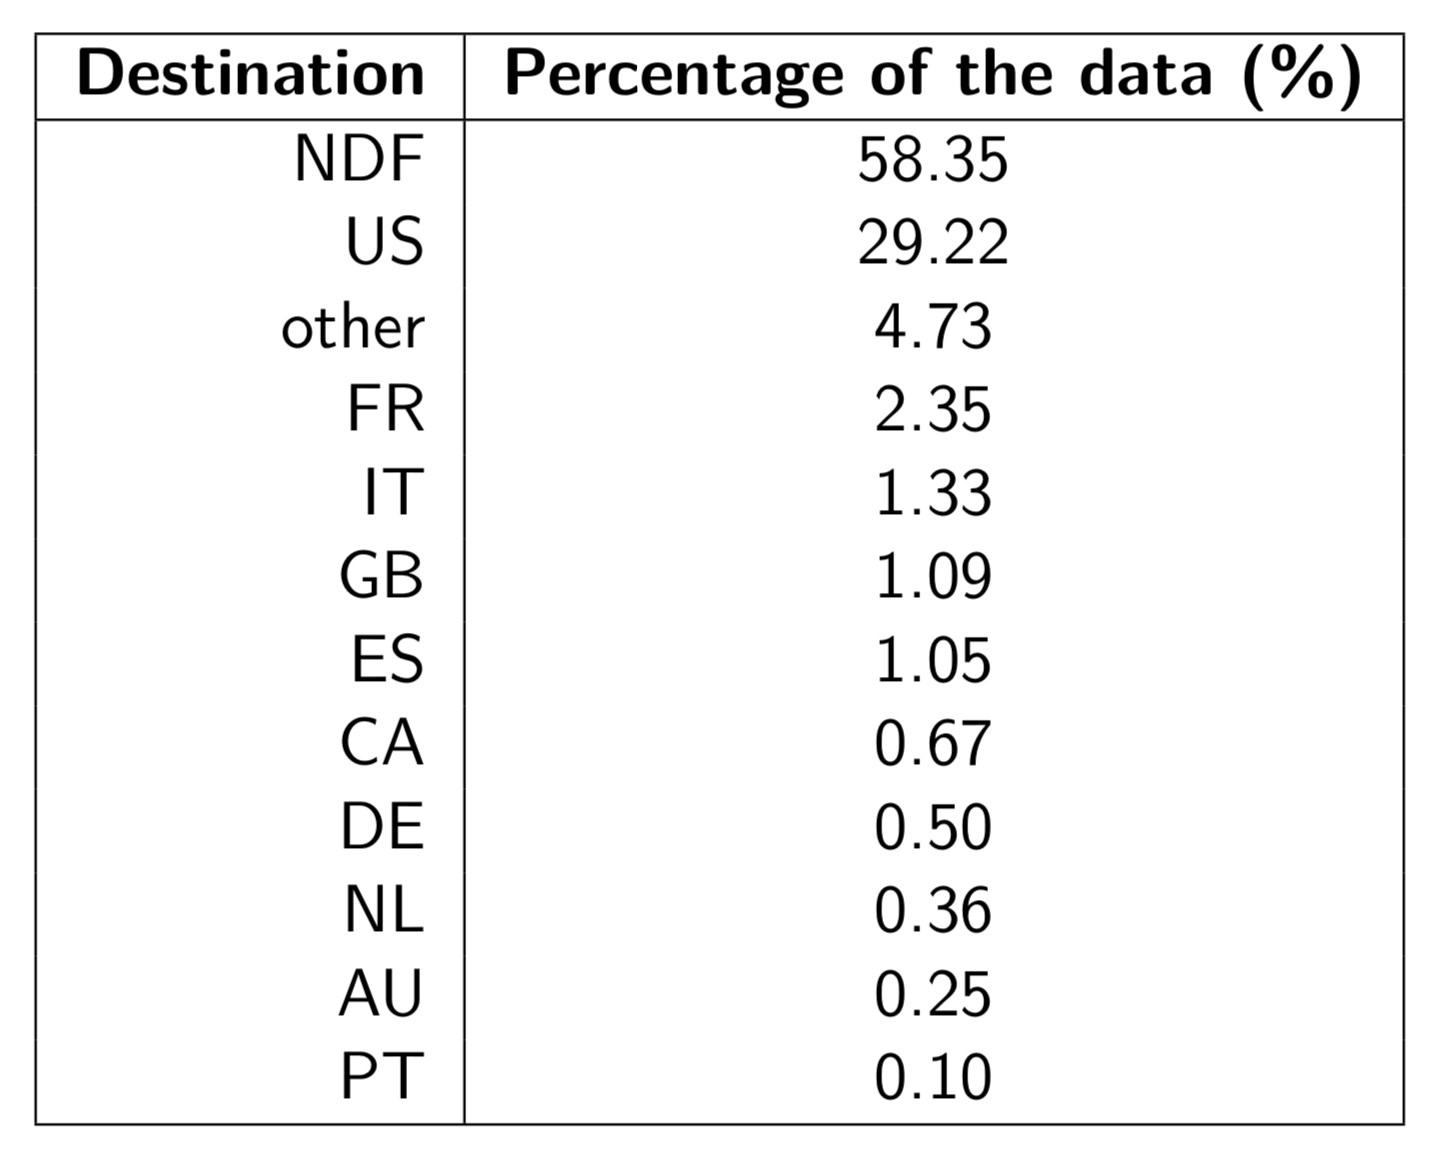
\includegraphics[width = 1.0\textwidth]{dest_table.png} 
        \caption{Percentage of bookings made to each destination}
      \end{figure}
  \end{column}
  \end{columns}
\end{frame}

% FEATURE IMPORTANCE ----------------------------------------------

\begin{frame}
\frametitle{Model Building: Feature Importance}
\begin{itemize}
  \item Full data was split into training (70\% of the data) and test sets
  \item 5-fold cross-validation was performed with XGBoost and random forest models, with just the top 200 most important features
  \item \textbf{Accuracy:} 87\%
  \item Both models only made predictions for US and NDF
\end{itemize}
\end{frame}

% FEATURE IMPORTANCE TABLE ----------------------------------------

\begin{frame}
\frametitle{Model Building: Feature Importance}
\begin{table}[ht]
\centering
\begin{tabular}{| l | l |}
  \hline
  \textbf{XGBoost} & \textbf{Random Forest} \\ 
  \hline
  firstbook\_y.1 & firstbook\_sn.1 \\
  age\_clean & firstbook\_wkd.1 \\
  signup\_flow & firstbook\_y.1 \\
  firstbook\_snspring & lag\_acb\_binNA \\
  affiliate\_channelother & lag\_acb\_bin.1..365. \\
  gender\_cleanFEMALE & firstbook m.1 \\
  gender\_cleanMALE & lag\_bts\_bin.1..1369. \\
  age\_bucket.1 & lag\_bts\_binNA \\
  lag\_acb\_bin.1..365. & firstbook\_snspring \\
  firstbook\_y2014 & firstbook y2013 \\
  \hline
\end{tabular}
\caption{Top 10 most important features for each model}
\end{table}
\end{frame}

% OVERSAMPLING ----------------------------------------------------

\begin{frame}
\frametitle{Model Building: Accounting for Imbalanced Classes}
\begin{itemize}
  \item Two techniques:
  \begin{itemize}
    \item Oversampling with replacement from under-represented destinations, under-sampling from over-represented destinations
    \item Synthetic Minority Oversampling Techniques (SMOTE) combined with under-sampling from over-represented destinations 
  \end{itemize}
  \item Under-represented destinations made up at least 4\% of the training data after oversampling
\end{itemize}
\end{frame}

% OVERSAMPLING RESULTS --------------------------------------------

\begin{frame}
\frametitle{Model Building: Results of Oversampling Techniques}
\begin{itemize}
  \item \textbf{Accuracy:} 87\%
\end{itemize}
\begin{figure}
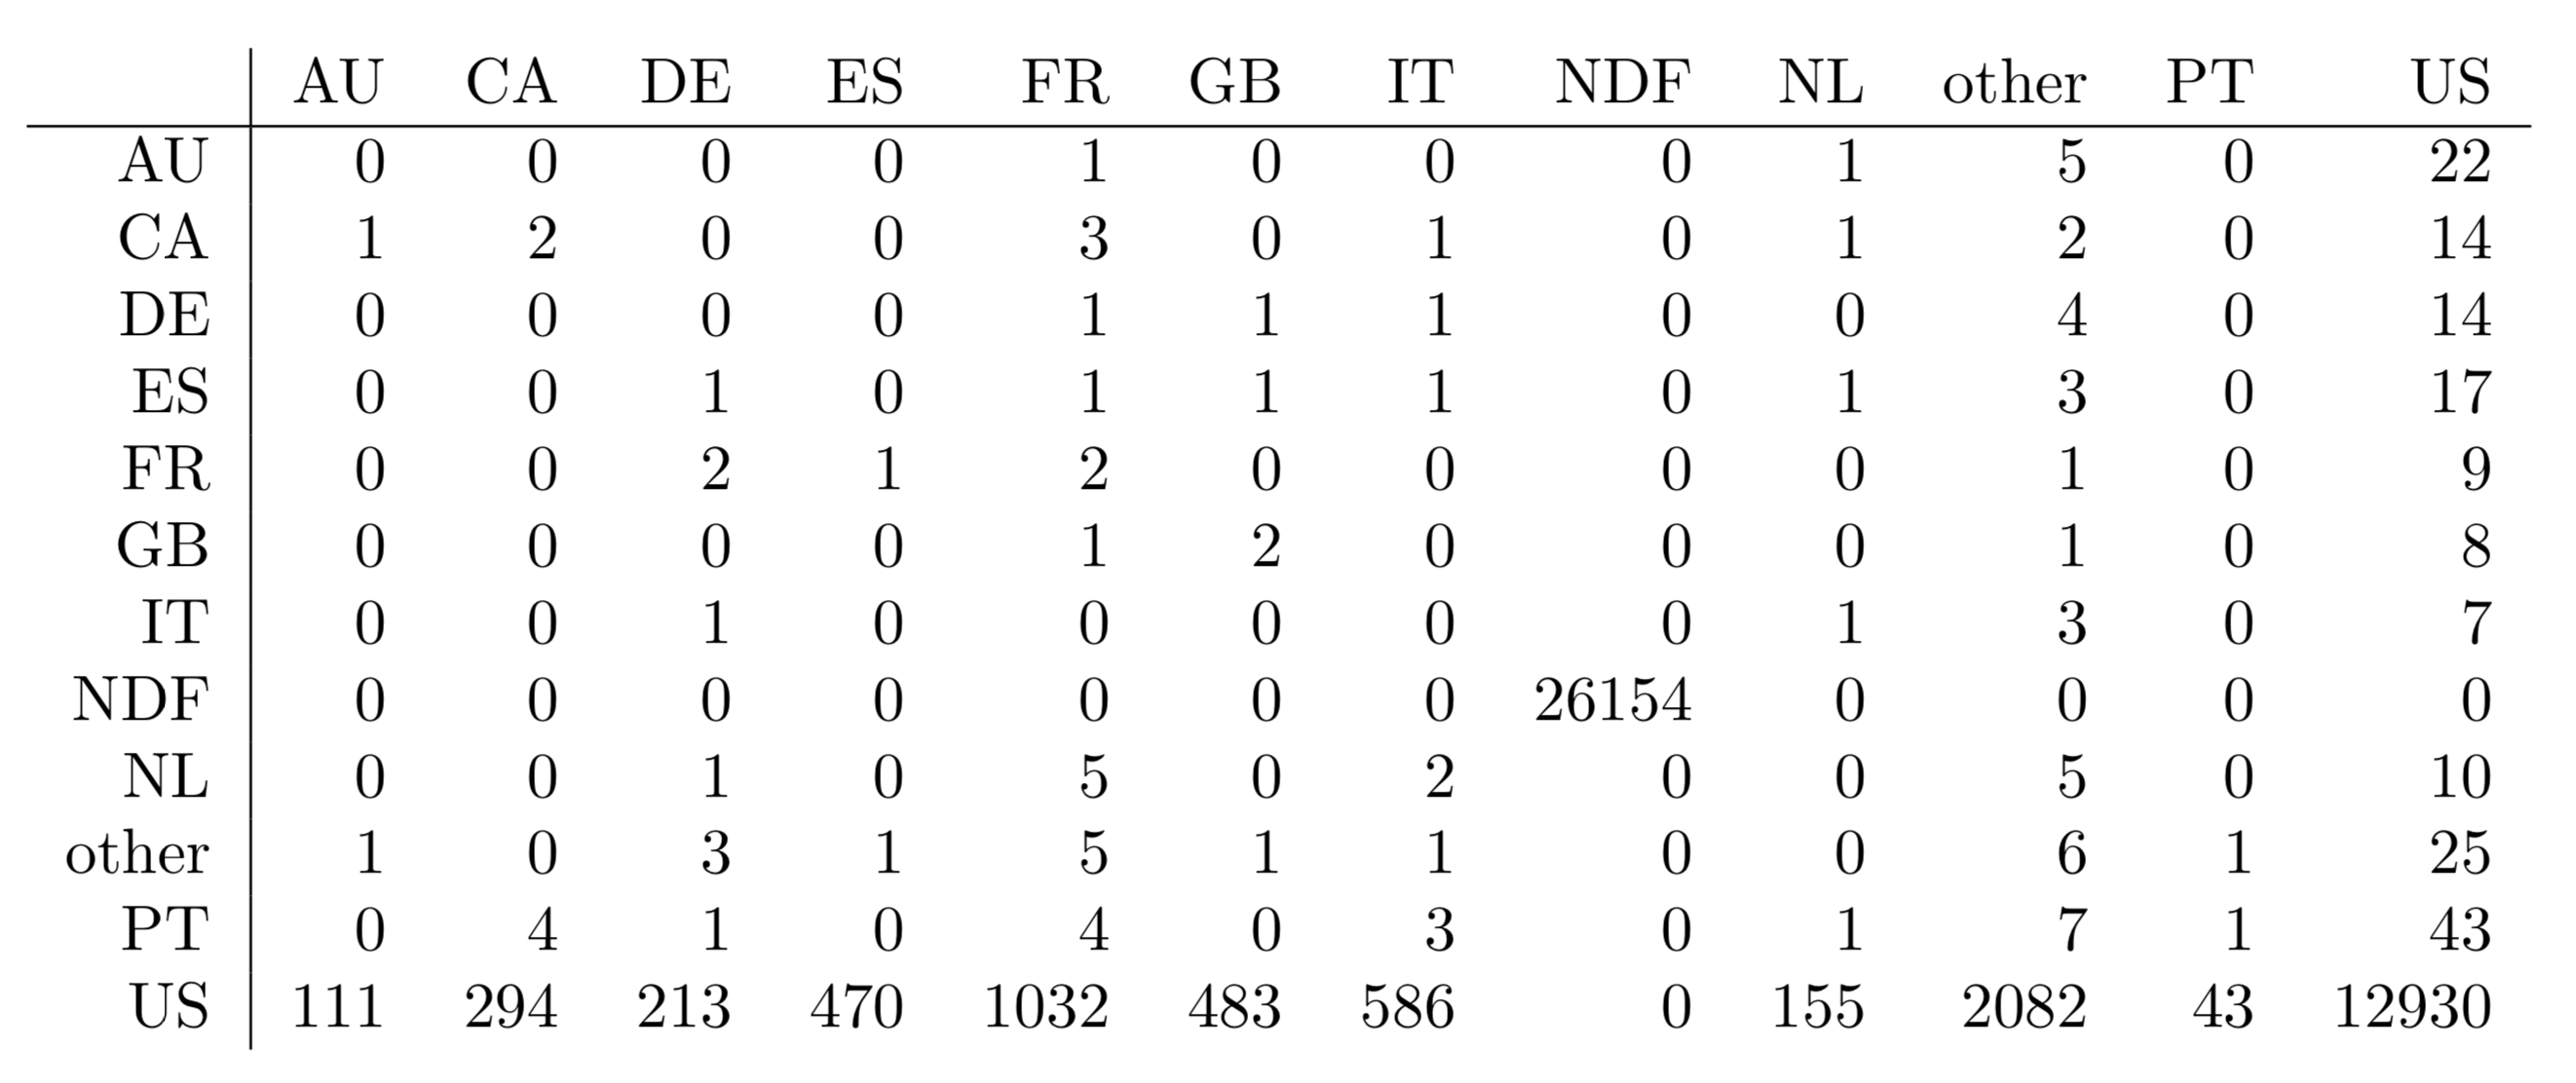
\includegraphics[width=1\linewidth]{confusion_matrix.png}
\caption{Confusion matrix of predictions made with XGBoost on the regular over-sampled training set}
\end{figure}
\end{frame}

% STACKED MODELING ------------------------------------------------

\begin{frame}
\frametitle{Model Building: Stacked Modeling}
\begin{itemize}
  \item Training data was partitioned into five folds, each containing 20\% of the data
  \item Build each model on four of the training folds, test on the held-out fold
  \item Repeated the process until each fold was used as a test fold
  \item Stored those predictions in two columns in the training set
  \item Fit each model to the full training set, predict on the test data, store predictions in the test set
  \item Final XGBoost fit to the predictions stored in the training set and tested on predictions stored in the test set 
\end{itemize}
\end{frame}

% RESULTS OF STACKING ---------------------------------------------

\begin{frame}
\frametitle{Model Building: Results of Stacking}
\begin{itemize}
  \item \textbf{Accuracy:} 87\%
\end{itemize}
\begin{figure}
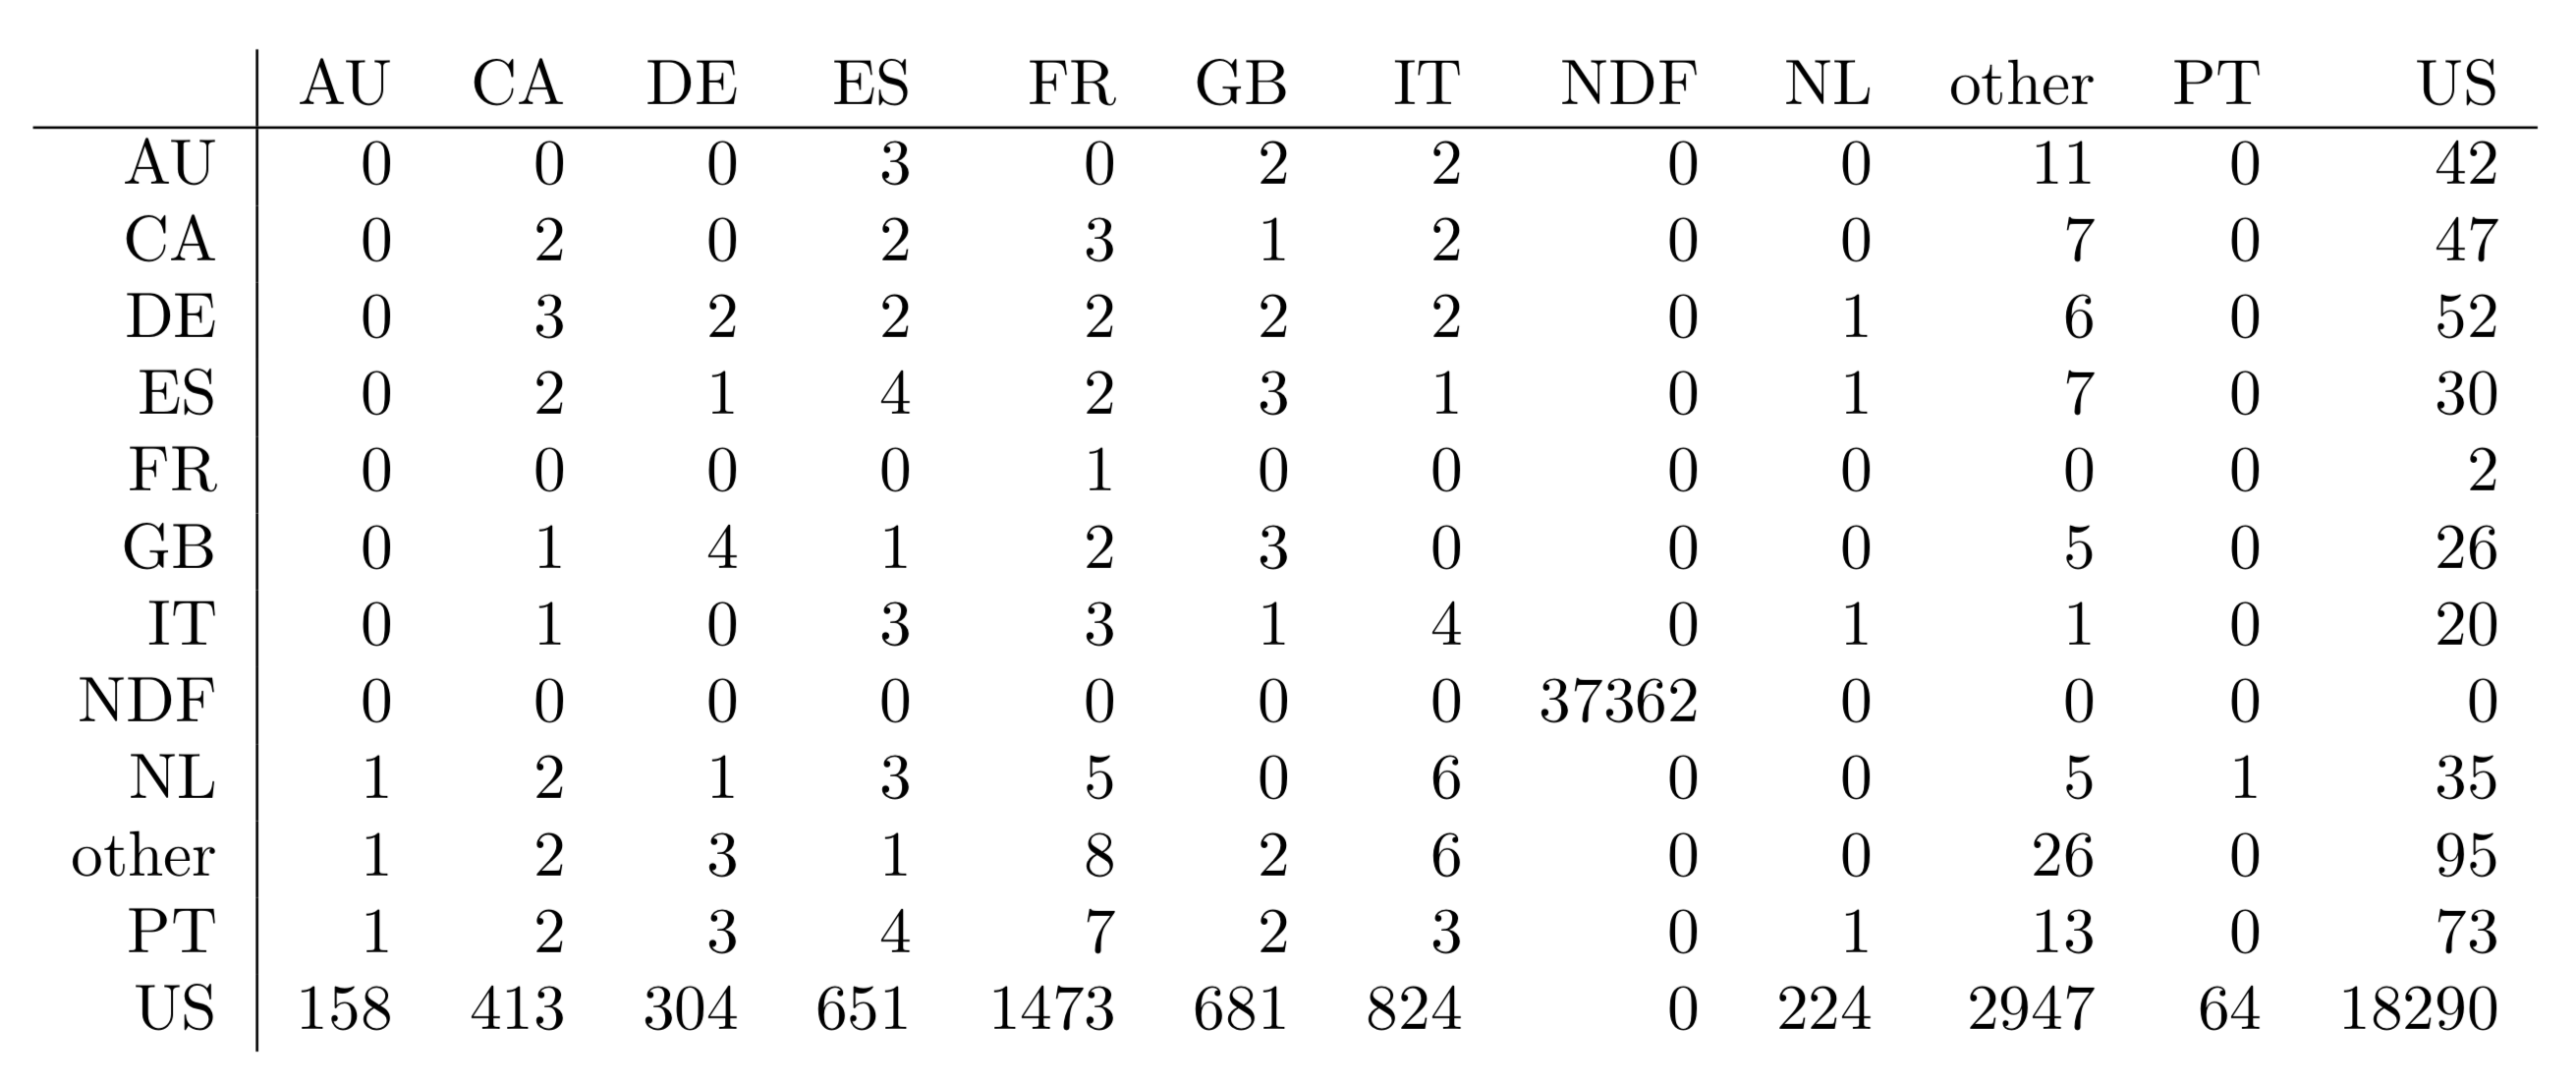
\includegraphics[width=1\linewidth]{stacked_confusion_m.png}
\caption{Confusion matrix of stacked model predictions, trained on the regular over-sampled training set}
\end{figure}
\end{frame}

% CV ON FULL DATA -------------------------------------------------

\begin{frame}
\frametitle{Model Building: Last Steps}
\begin{itemize}
  \item Perform five-fold cross-validation with XGBoost, random forest, and stacked model on the full data 
  \item \textbf{Accuracy:} 87\%
  \item Run times: 
  \begin{itemize}
    \item Random forest: 27.5 min
    \item XGBoost: 28.7 min
    \item Stacked model: 3.24 hr
  \end{itemize}
\end{itemize}
\end{frame}

% MODEL PERFORMANCE DISCUSSION ------------------------------------

\begin{frame}
\frametitle{Discussion: Model Performance}
\begin{itemize}
  \item Extremely imbalanced classes
  \item Base classifiers of the stacked model performed poorly in similar ways
\end{itemize}
\end{frame}

% NEXT STEPS ------------------------------------------------------

\begin{frame}
\frametitle{Discussion: Next Steps}
\begin{itemize}
  \item Stack more than two models 
  \item Build additional models to predict missing values for certain variables
  \item Incorporate the other available data sets 
  \item Parameter tuning
\end{itemize}
\end{frame}

% END -------------------------------------------------------------

\begin{frame}
Thank you!
\end{frame}


\end{document}
